\documentclass{beamer}
\usepackage[table]{}
\usepackage{emoji}

\usepackage{hyperref}
\usepackage{graphicx}
\usepackage{amsmath}
\usepackage{tcolorbox}

\usepackage{tabularx}
\usepackage{colortbl}
\usepackage{multirow}
\usepackage{caption}


\addtobeamertemplate{background canvas}{\transfade[duration=0.8]}{}


\beamertemplatenavigationsymbolsempty
\setbeamertemplate{frametitle}[default][center]

\usepackage{xcolor}
\definecolor{mbrown}{RGB}{106, 72, 10}

\usetheme{Singapore}
\usecolortheme[named=mbrown]{structure}

\hypersetup{
    colorlinks=true,
    linkcolor=blue, % Color of internal links
    urlcolor=blue   % Color of external links
}
\date{October 3 2023}
\begin{document}

\begin{frame}{Doubly Fed Induction Generator}
\centering By Adhithya
\begin{figure}
    \centering
    \fbox{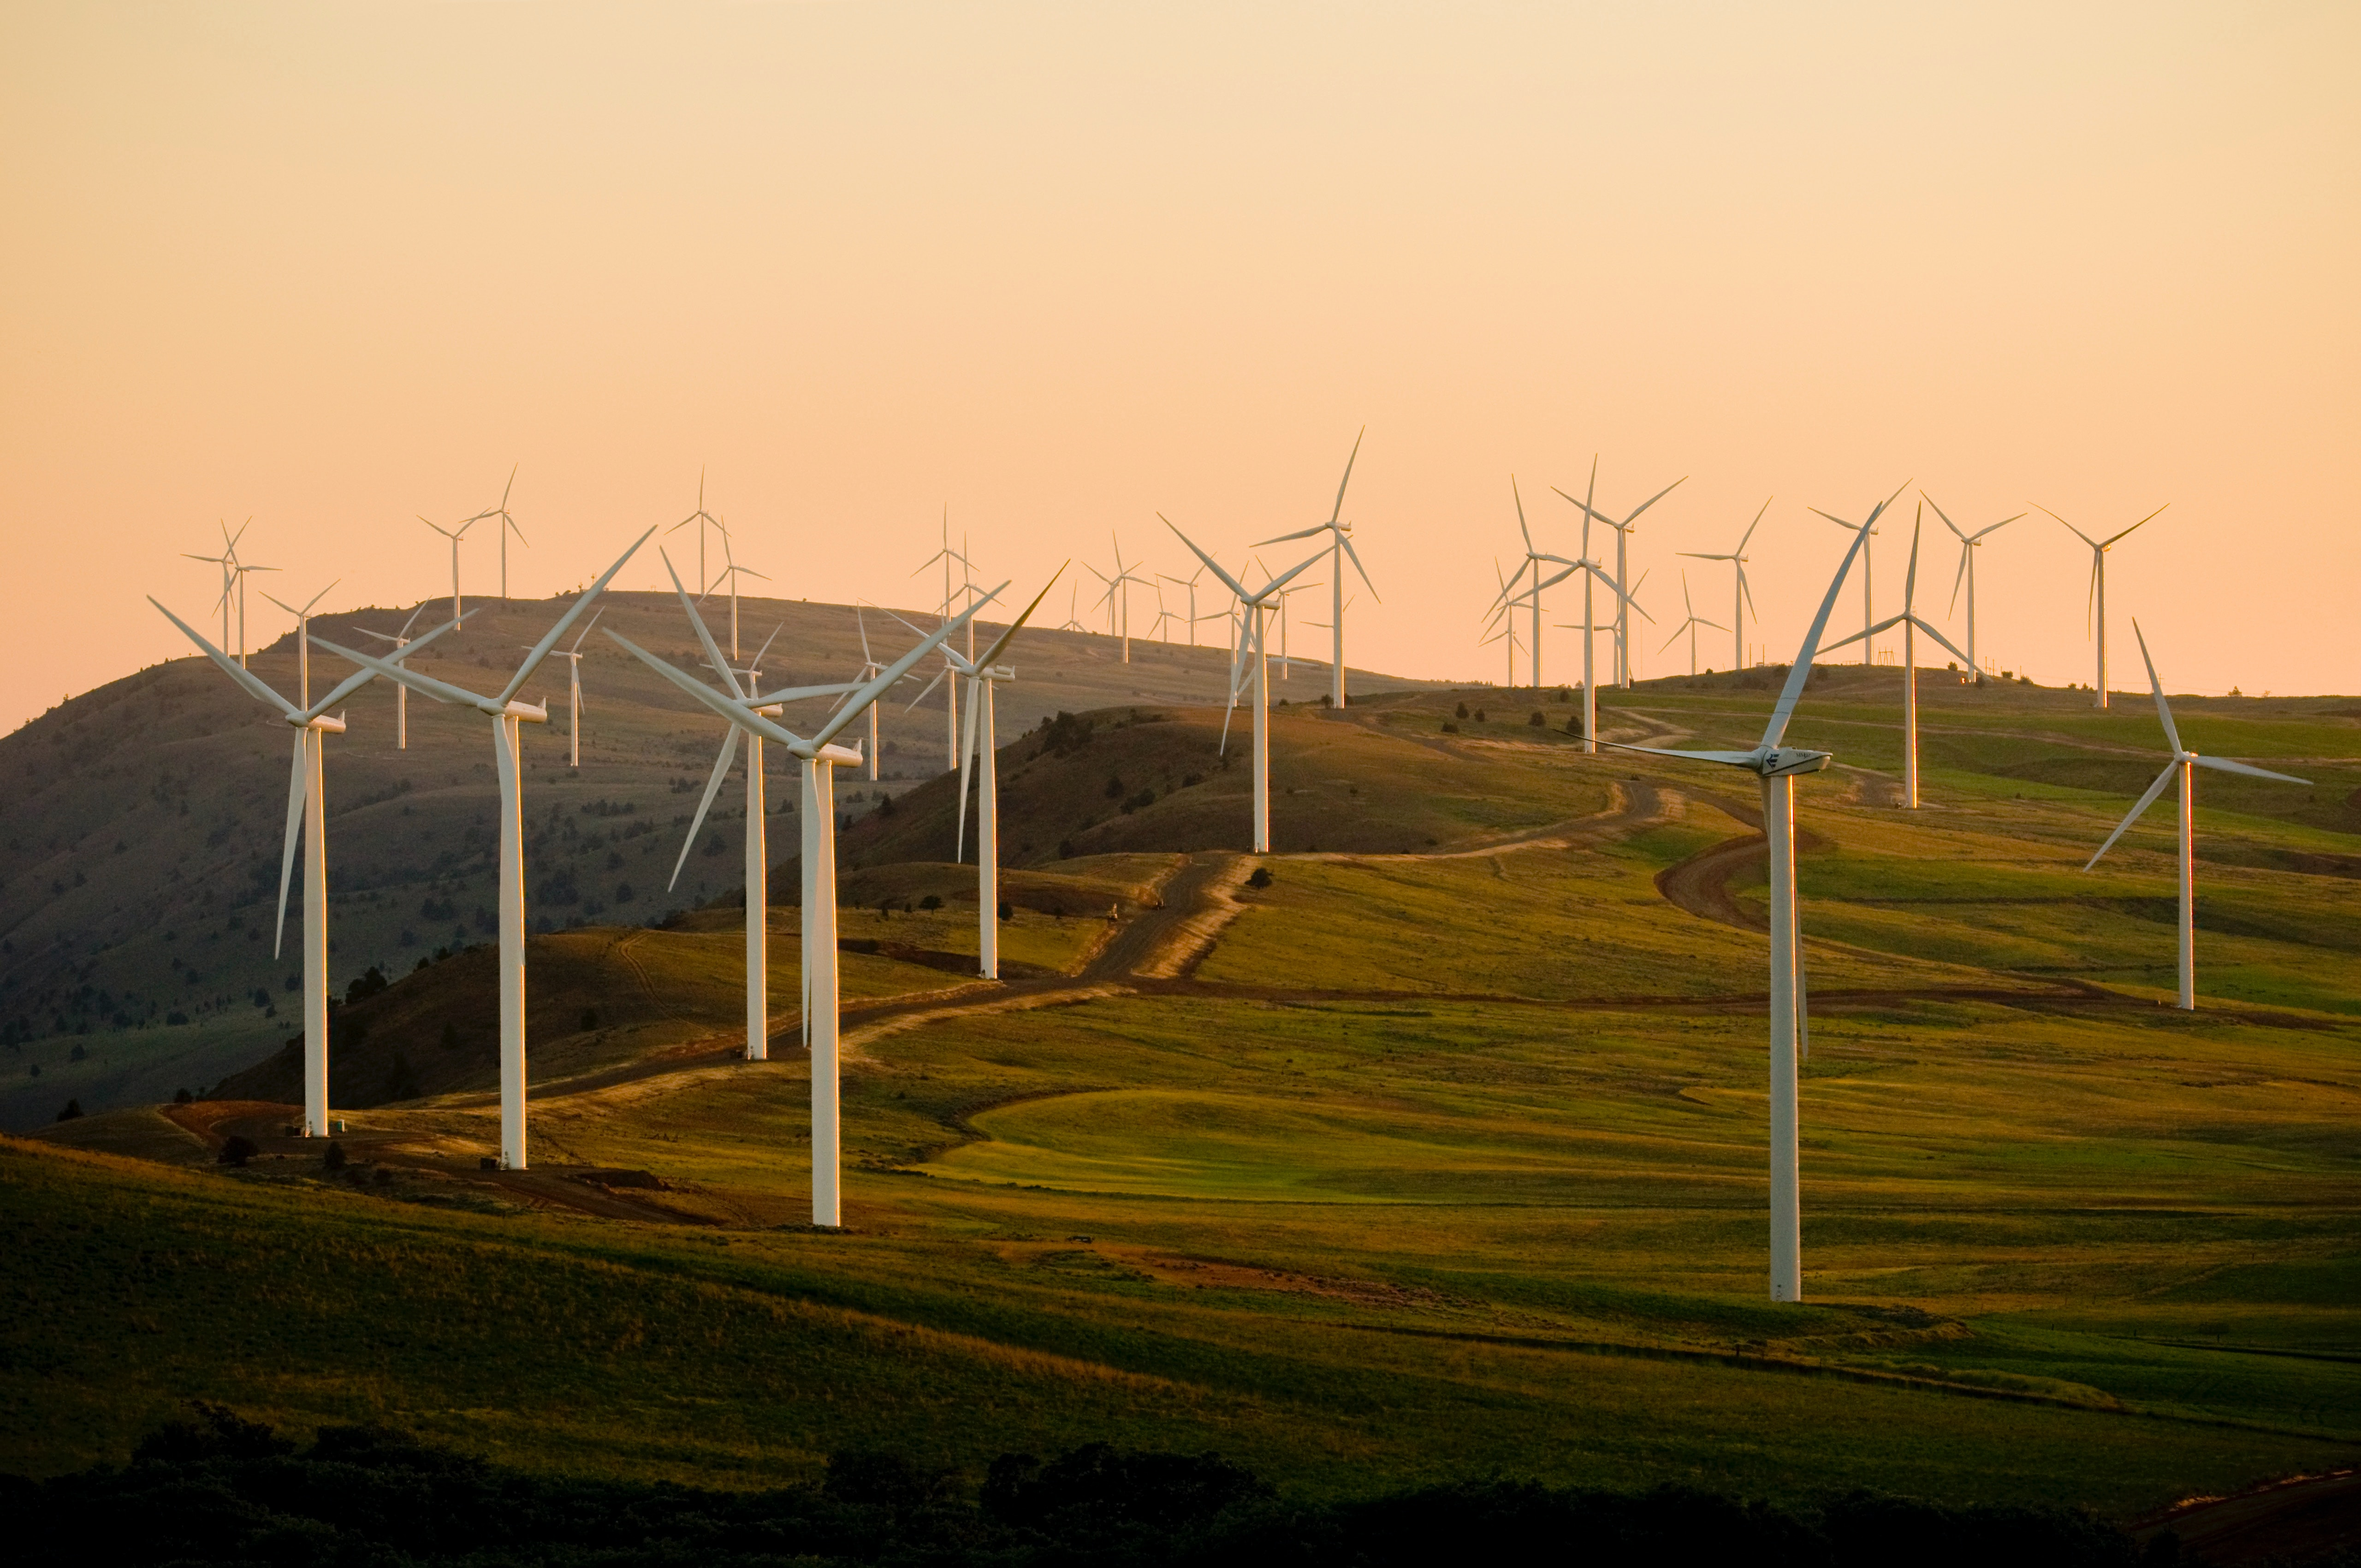
\includegraphics[width=3.5in]{imgs/windFarm.jpg}}
\end{figure}
\end{frame}

\section{Structure of DFIG}

\begin{frame}{What is a DFIG?}
  \begin{columns}
    \begin{column}{0.6\textwidth} 
    \begin{figure}
        \centering
        \fbox{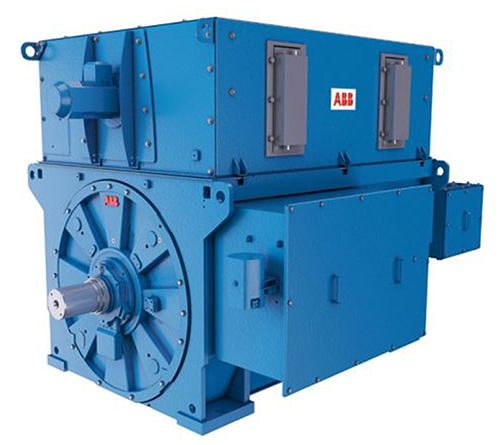
\includegraphics[width=2.2in]{imgs/ABB.png}}
        \caption{Commercially available DFIG.
        \textit{Courtesy of ABB}}
    \end{figure}
    \end{column}
    
    \begin{column}{0.4\textwidth} % Adjust the width as needed
      \begin{itemize}
        \item It has two sets of $\textcolor{red!70!black}{3} \, \textcolor{yellow!50!black}{\phi} \, \textcolor{blue!70!black}{windings}$: on both \textbf{stator} and \textbf{rotor}.
        
        \item Suited for \textbf{variable speed} common which is common with wind turbines.
      \end{itemize}
    \end{column}
  \end{columns}
\end{frame}


\begin{frame}{Technical Specification}
  
  \begin{columns}
  
        \begin{column}{0.4\textwidth} % Adjust the width as needed
    \begin{figure}
        \centering
        \fbox{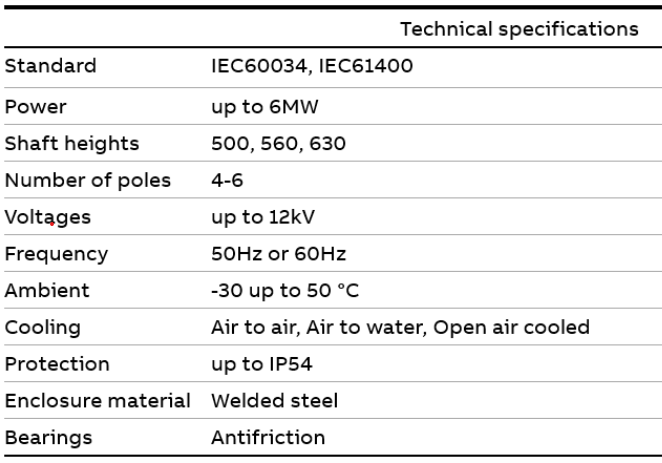
\includegraphics[width=2.0in]{imgs/spec.png}}
        \caption{Nameplate details.}
    \end{figure}
    \end{column}
    
    \begin{column}{0.6\textwidth} 
    \begin{figure}
        \centering
        \fbox{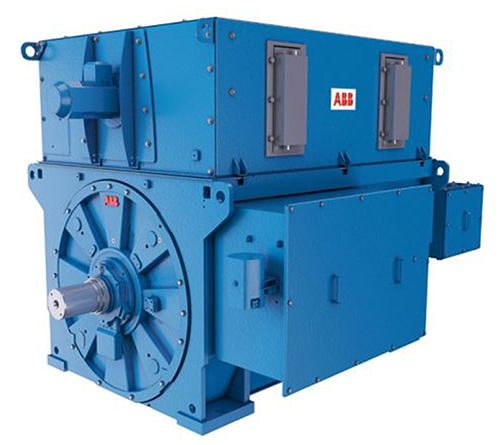
\includegraphics[width=2in]{imgs/ABB.png}}
    \end{figure}
    \end{column}

  \end{columns}
\end{frame}




\begin{frame}{Antifriction bearing}

    \begin{figure}
        \centering
        \fbox{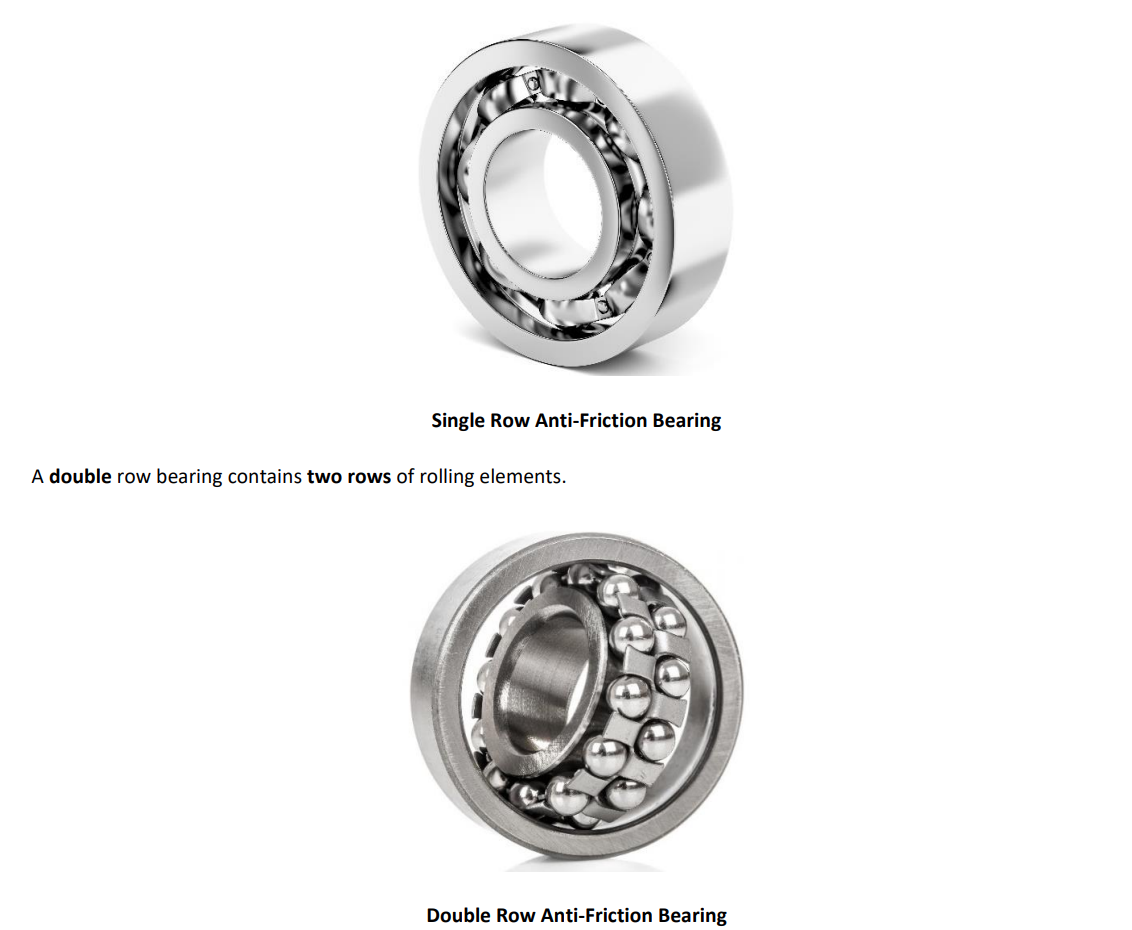
\includegraphics[width=2.8in]{imgs/antiFriction.png}}
        \caption{Image Courtesy of cedengineering.com}
    \end{figure}    
\end{frame}

\begin{frame}{Stator}
        \begin{figure}
        \centering
        \fbox{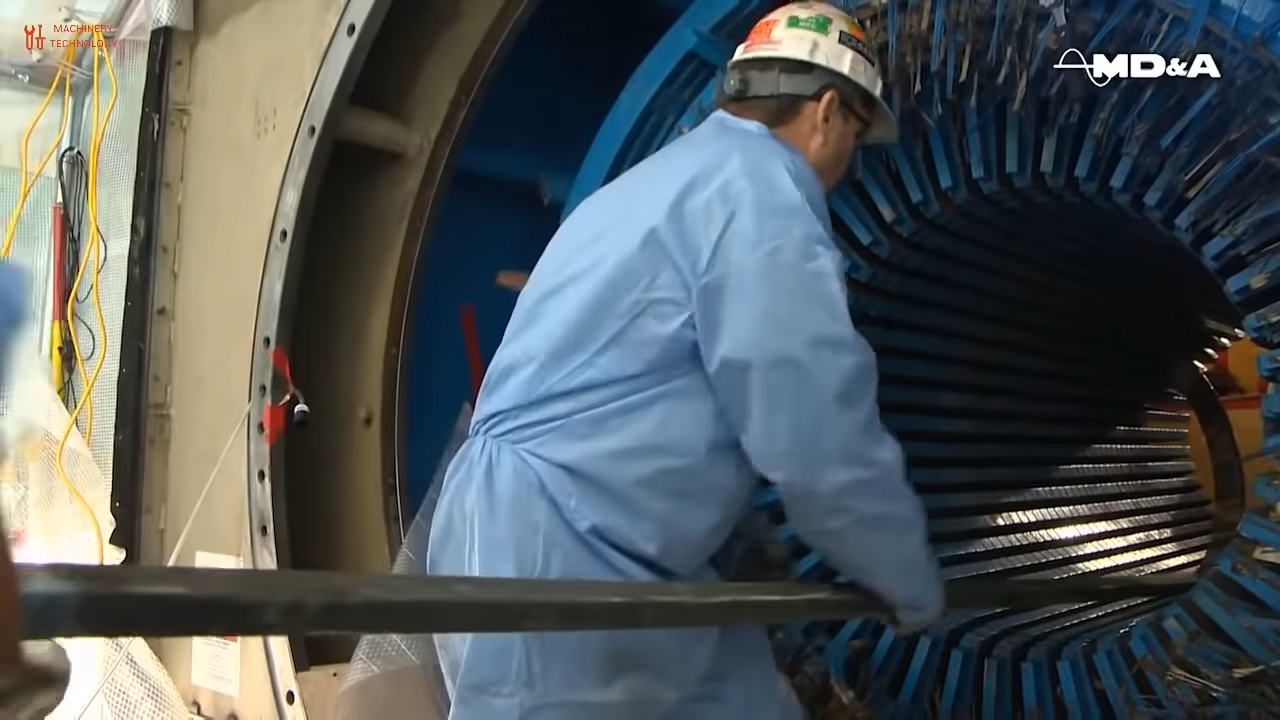
\includegraphics[width=3.7in]{imgs/stator.png}}
        \caption{Typical large $\textcolor{red!70!black}{3} \, \textcolor{yellow!50!black}{\phi} \, \textcolor{blue!70!black}{stator}.$}
    \end{figure}
\end{frame}

\begin{frame}{Rotor}
  \begin{minipage}{0.48\textwidth}
    \centering
    \begin{figure}
      \fbox{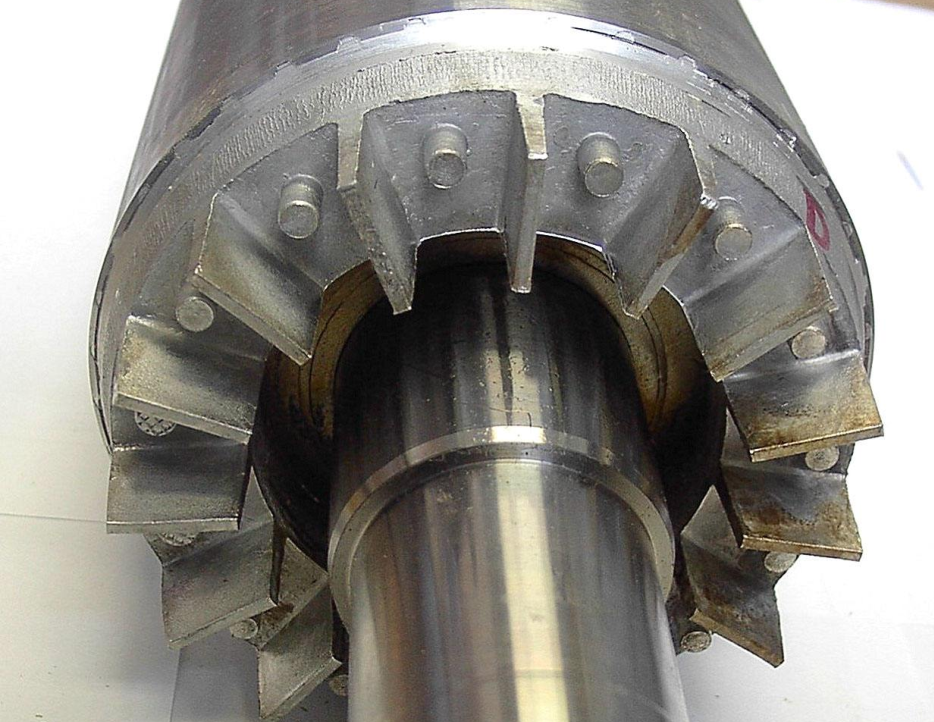
\includegraphics[width=\linewidth]{imgs/sqCageRotor.png}}
      \caption{Squirrel Cage}
    \end{figure}
  \end{minipage}\hfill
  \begin{minipage}{0.48\textwidth}
    \centering
    \begin{figure}
      \fbox{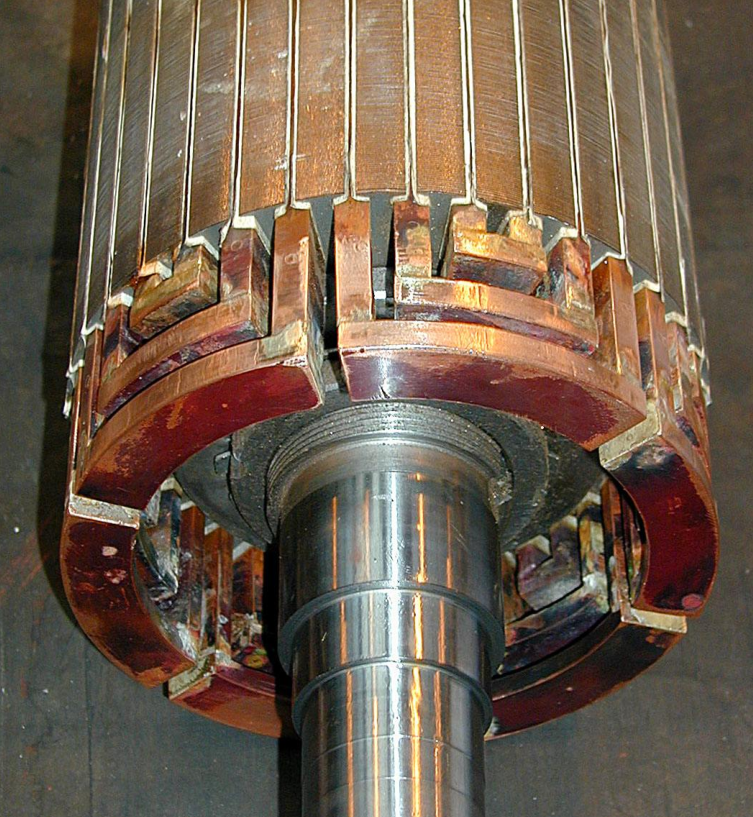
\includegraphics[width=0.7\linewidth]{imgs/rotor1.png}}
      \caption{Wound Rotor}
    \end{figure}
  \end{minipage}
\end{frame}


\begin{frame}{Rotor}

    \begin{figure}
        \centering
        \fbox{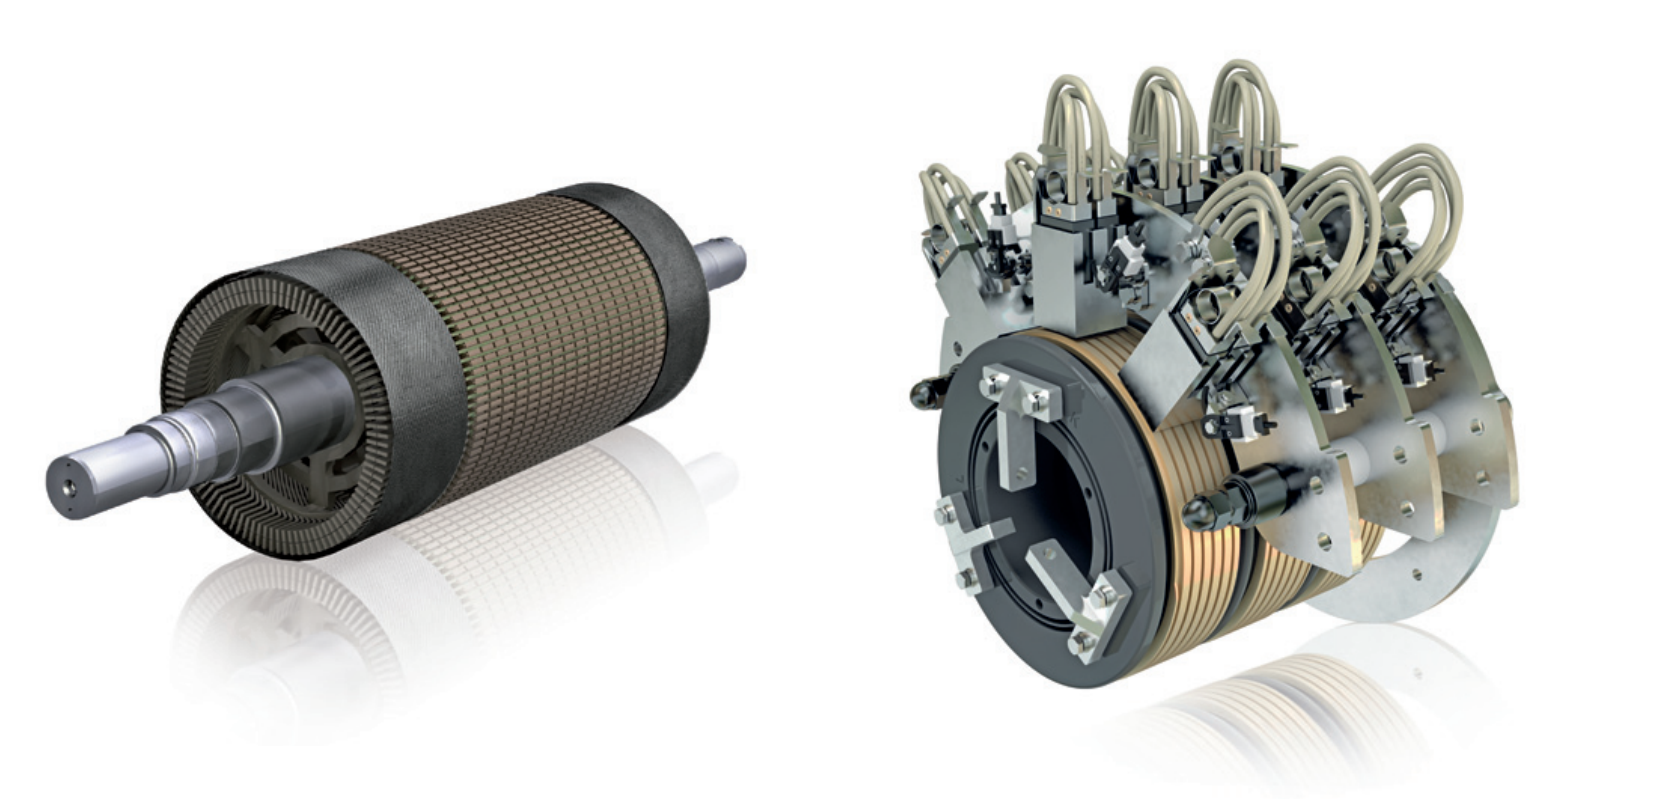
\includegraphics[width=3.9in]{imgs/rotorSlipRings.png}}
        \caption{Image courtesy of ABB}
    \end{figure}    
\end{frame}


\begin{frame}{Rotor details}
  
  \begin{columns}
  
        \begin{column}{0.6\textwidth} % Adjust the width as needed
    \begin{figure}
        \centering
        \fbox{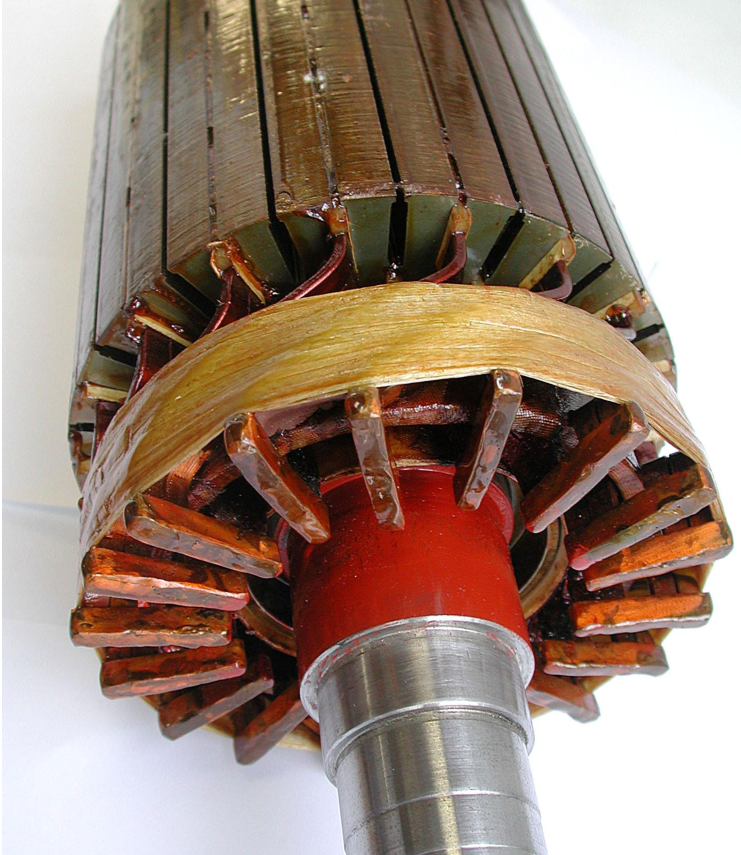
\includegraphics[width=2.0in]{imgs/rotor.png}}
        \caption{\small DFIG Rotor.}
    \end{figure}
    \end{column}
    
    \begin{column}{0.4\textwidth} 
        \begin{itemize}
            \item Rotor have high turns $(2\times\, to \,3\times)$ that of stator.

            \item Consequently, the rotor will have higher voltages and lower currents
        \end{itemize}
    \end{column}

  \end{columns}
\end{frame}


\section{DFIG System}

\begin{frame}{}
       \begin{figure}
        \centering
        \fbox{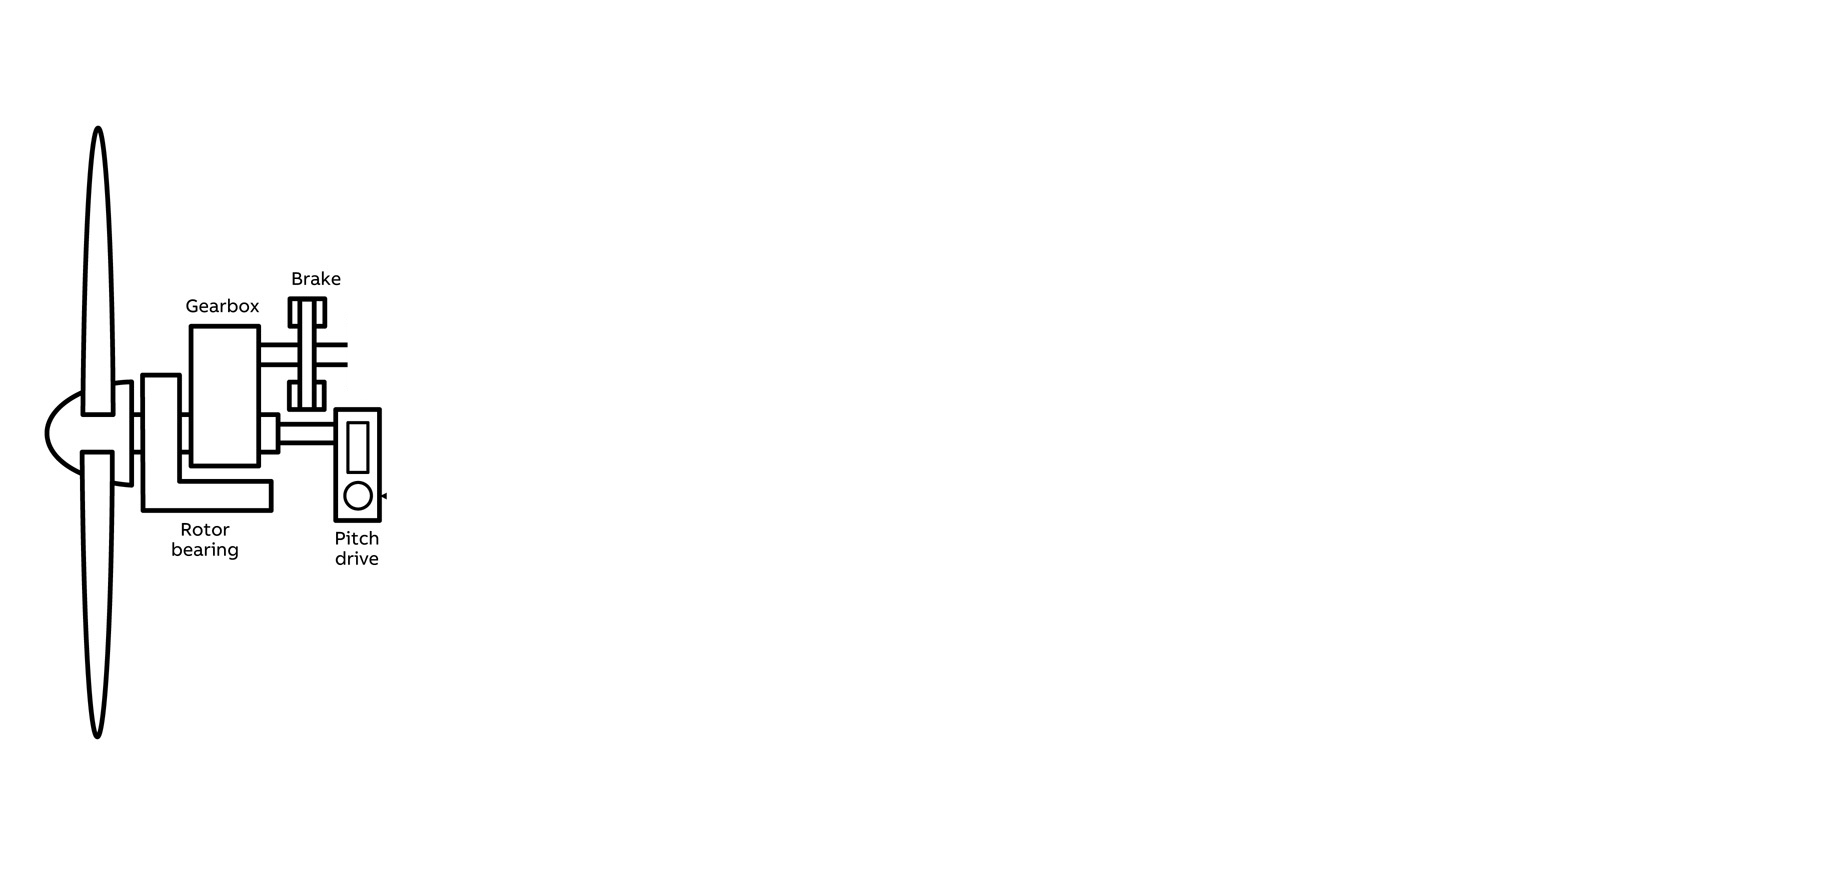
\includegraphics[width=4.5in]{imgs/working (2).jpg}}
        \caption{Prime Mover and it's auxiliaries.}
    \end{figure}
\end{frame}

\begin{frame}{}
       \begin{figure}
        \centering
        \fbox{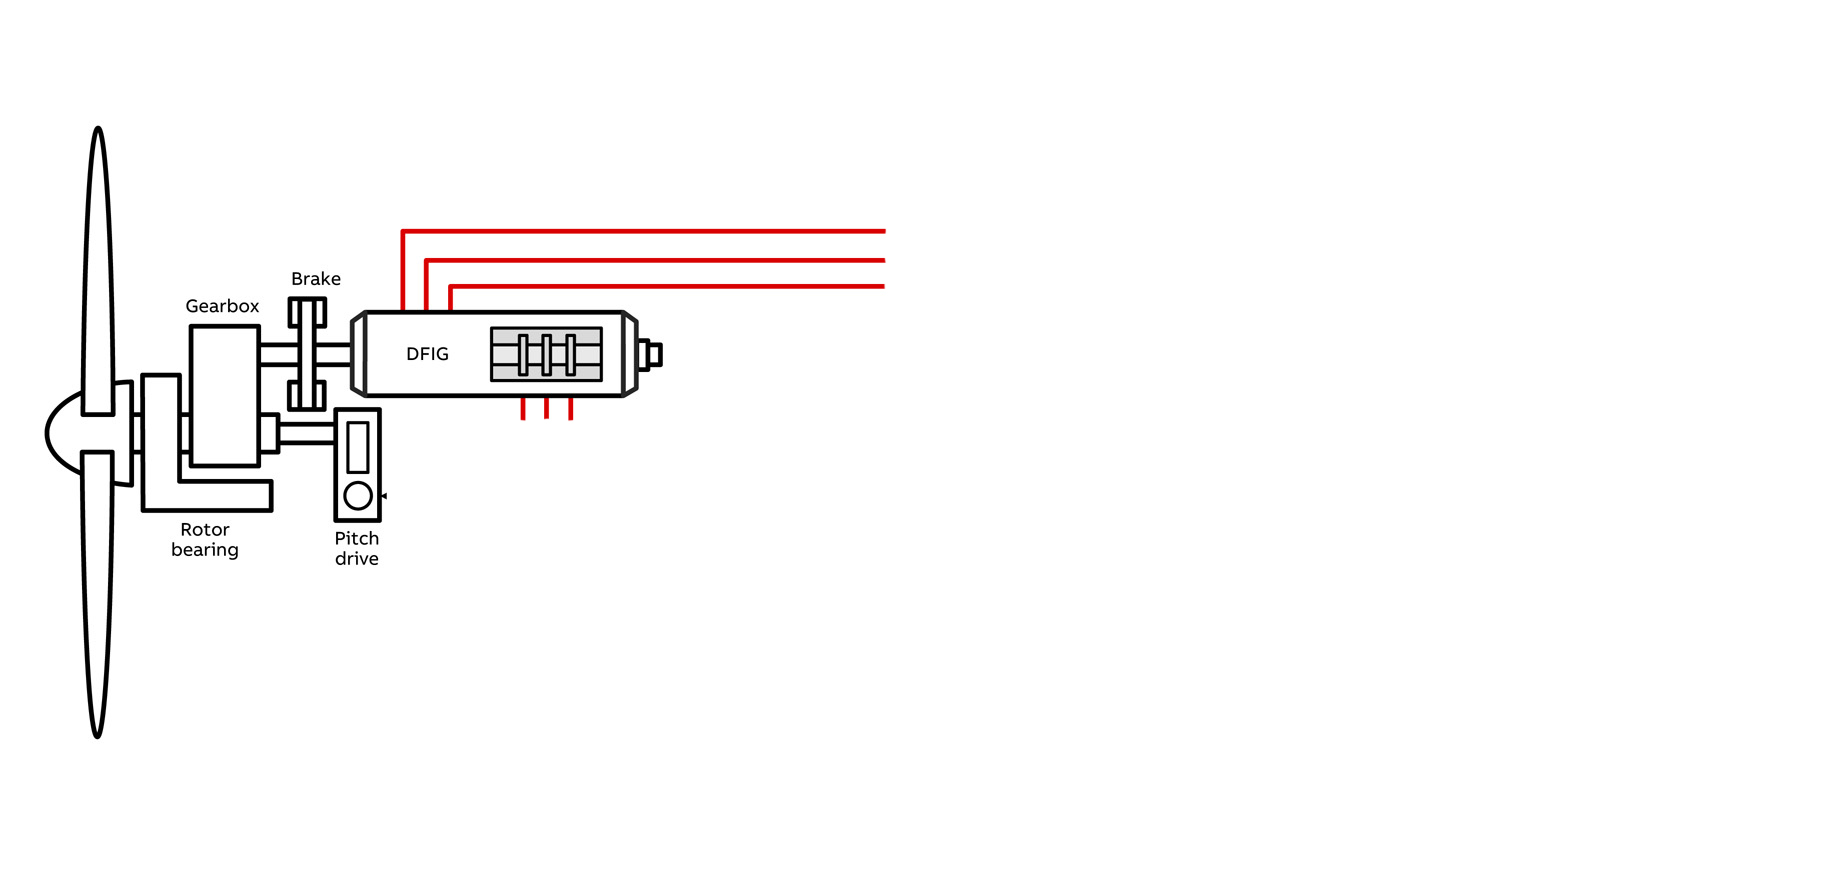
\includegraphics[width=4.5in]{imgs/working (3).jpg}}
        \caption{Generator}
    \end{figure}
\end{frame}

\begin{frame}{}
       \begin{figure}
        \centering
        \fbox{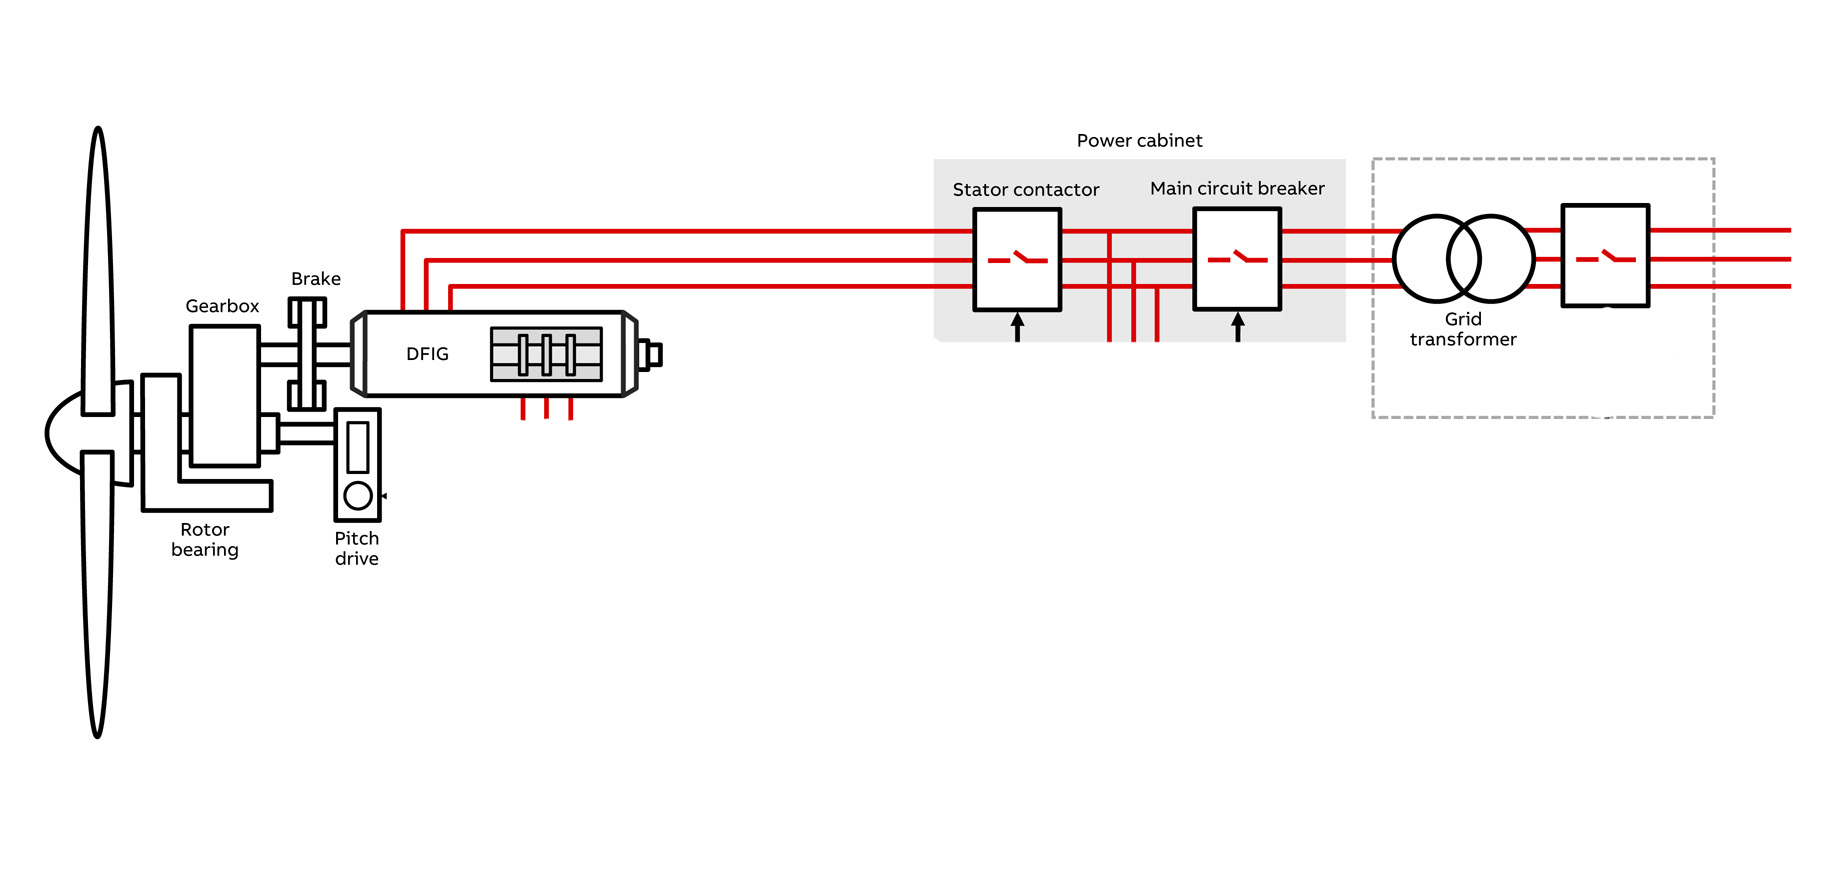
\includegraphics[width=4.5in]{imgs/working (4).jpg}}
        \caption{Stator Connections}
    \end{figure}
\end{frame}

\begin{frame}{}
       \begin{figure}
        \centering
        \fbox{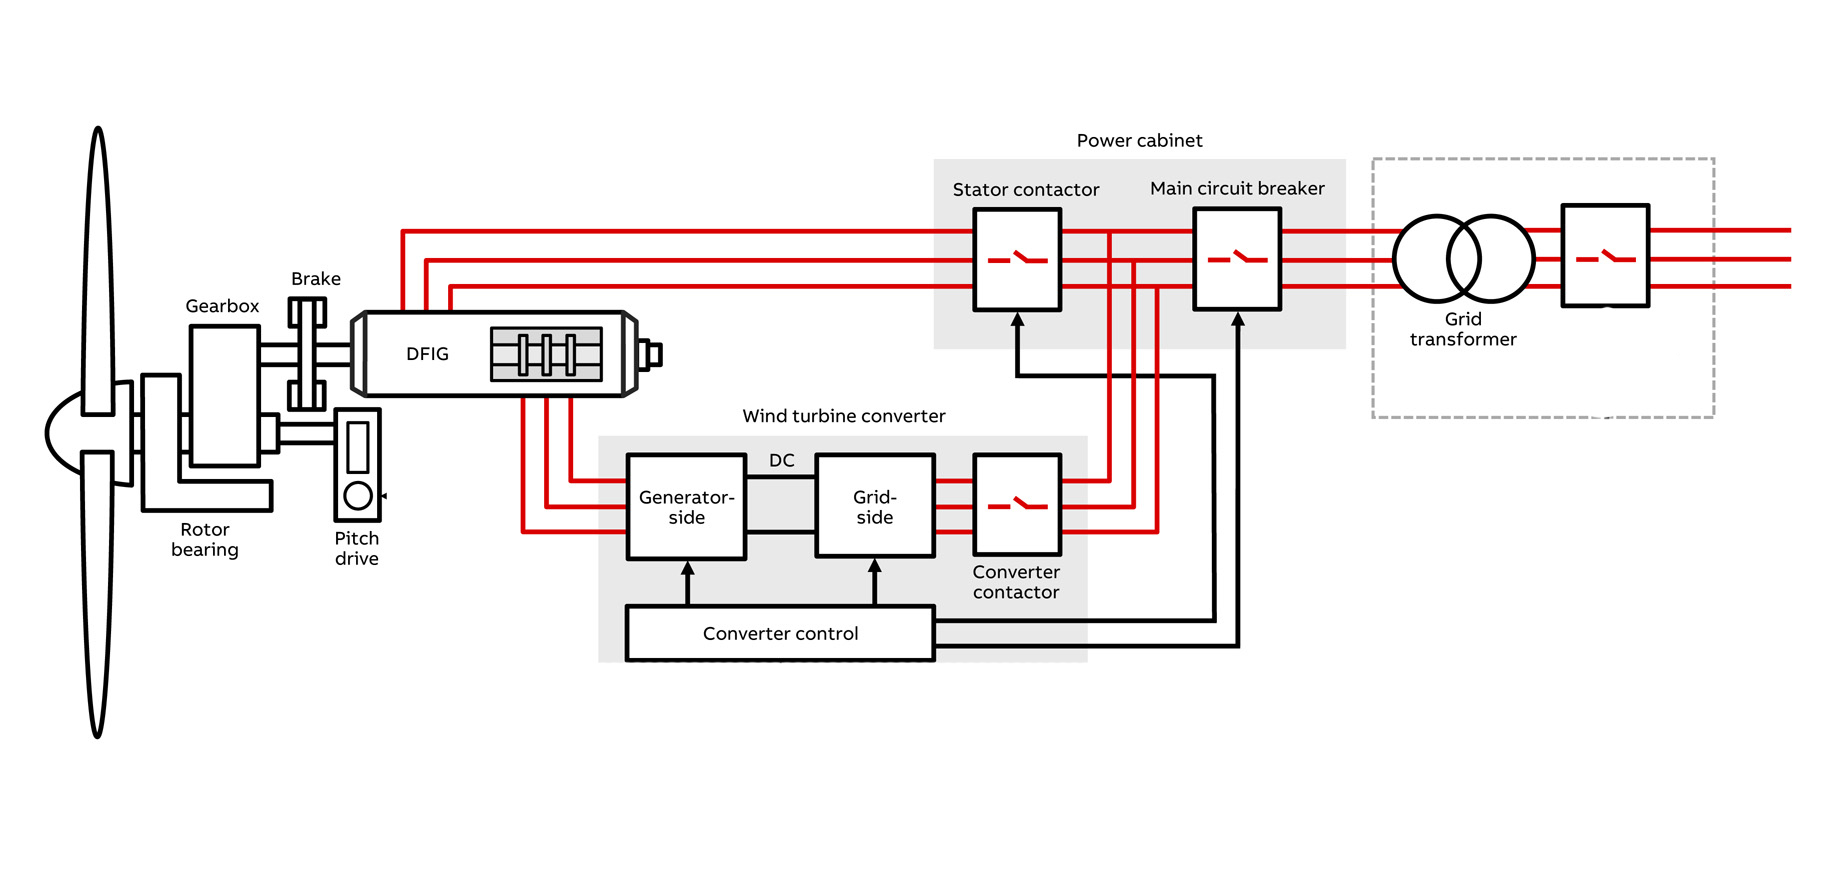
\includegraphics[width=4.5in]{imgs/working (5).jpg}}
        \caption{Rotor Connections and control}
    \end{figure}
\end{frame}

\begin{frame}{}
       \begin{figure}
        \centering
        \fbox{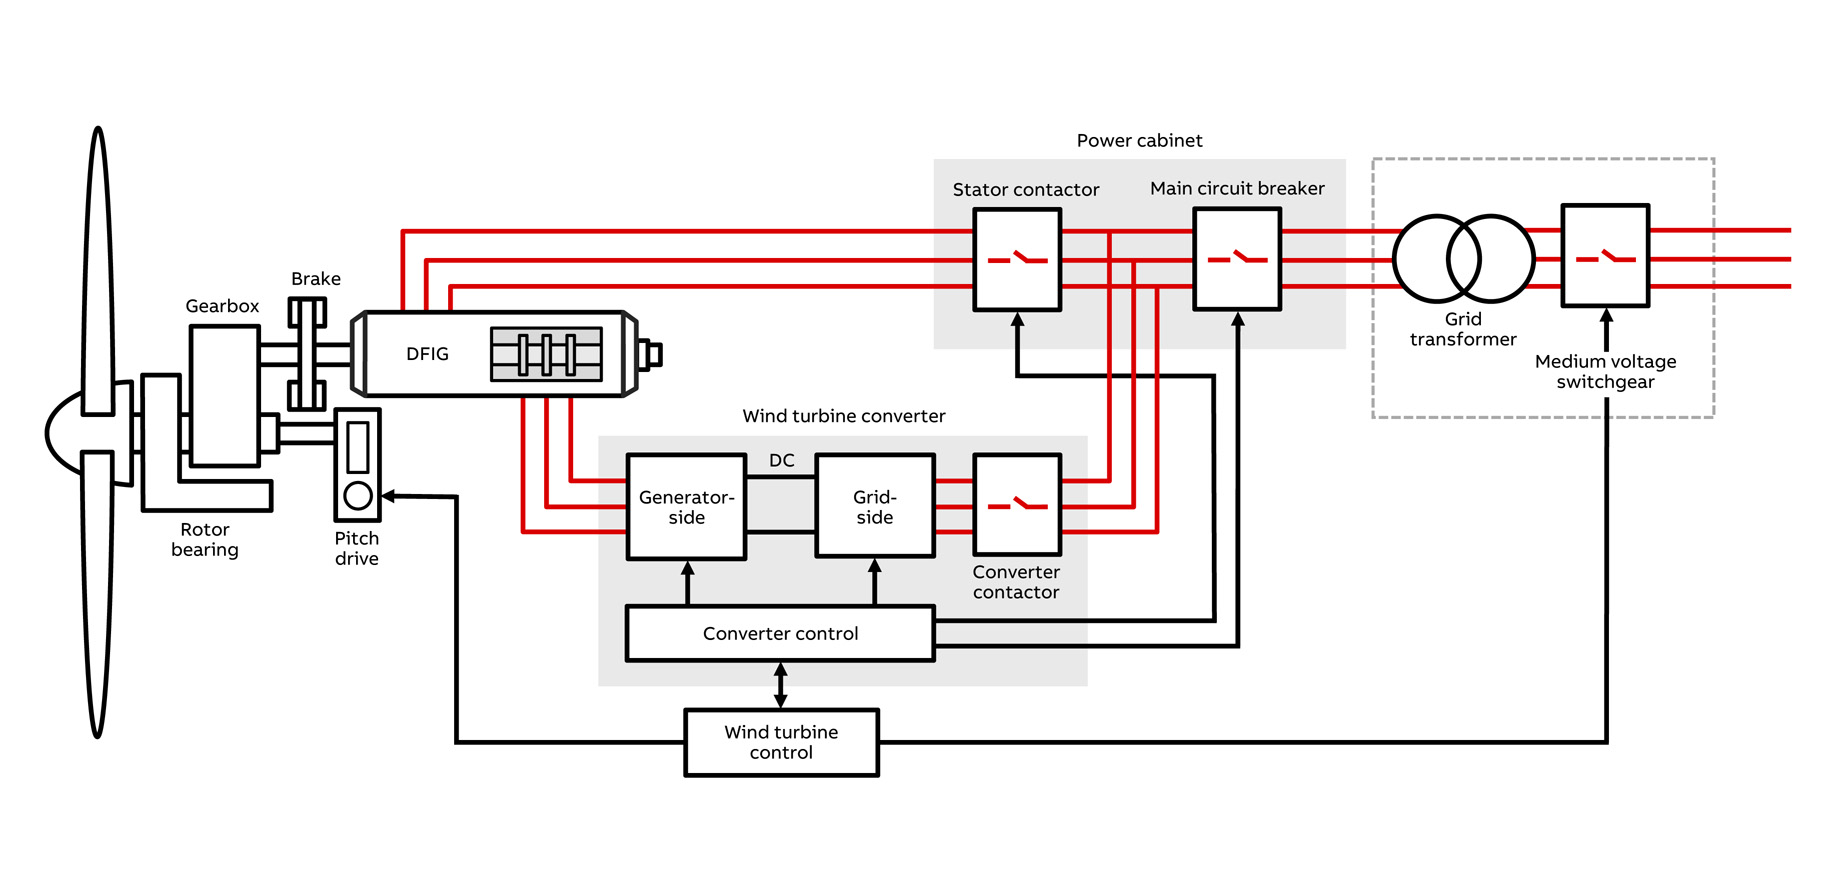
\includegraphics[width=4.5in]{imgs/DFIG.jpg}}
        \caption{DFIG system as a Whole.}
    \end{figure}
\end{frame}


\section{Variable Speed Operation}
\begin{frame}{Working}
    \begin{figure}
        \centering
        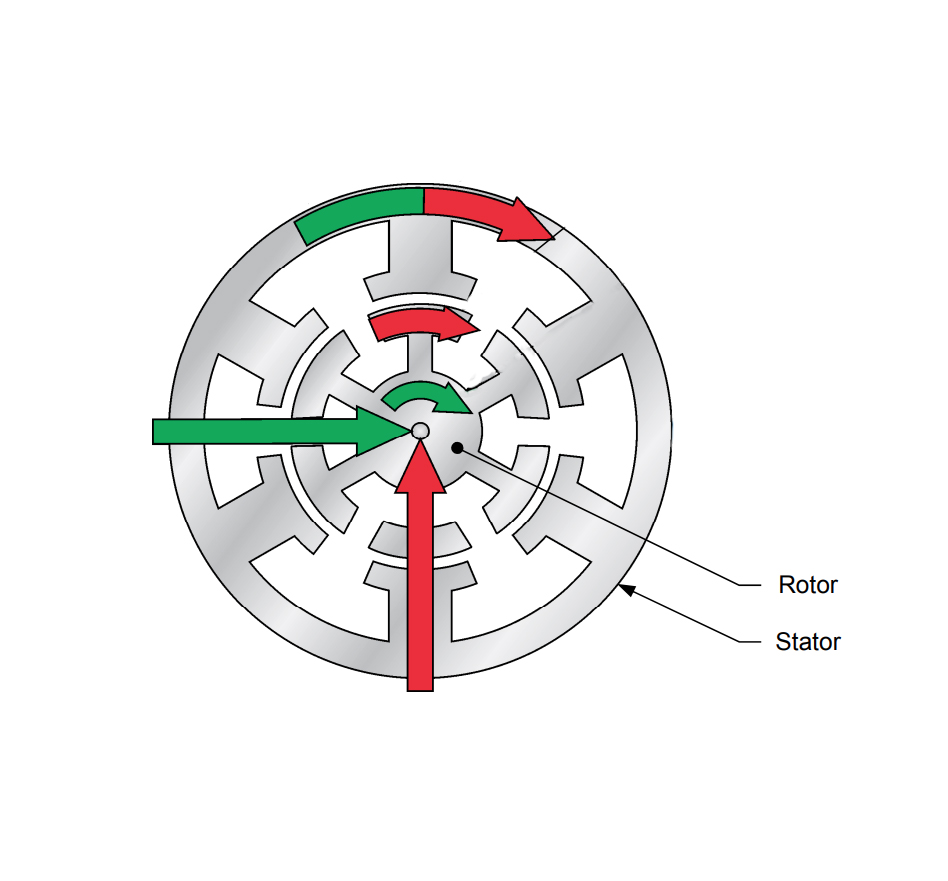
\includegraphics[width=2.85in]{imgs/dfigOP (1).jpg}
        \caption{Stator and Rotor of DFIG}
    \end{figure}
\end{frame}

\begin{frame}{}
    \begin{figure}
        \centering
        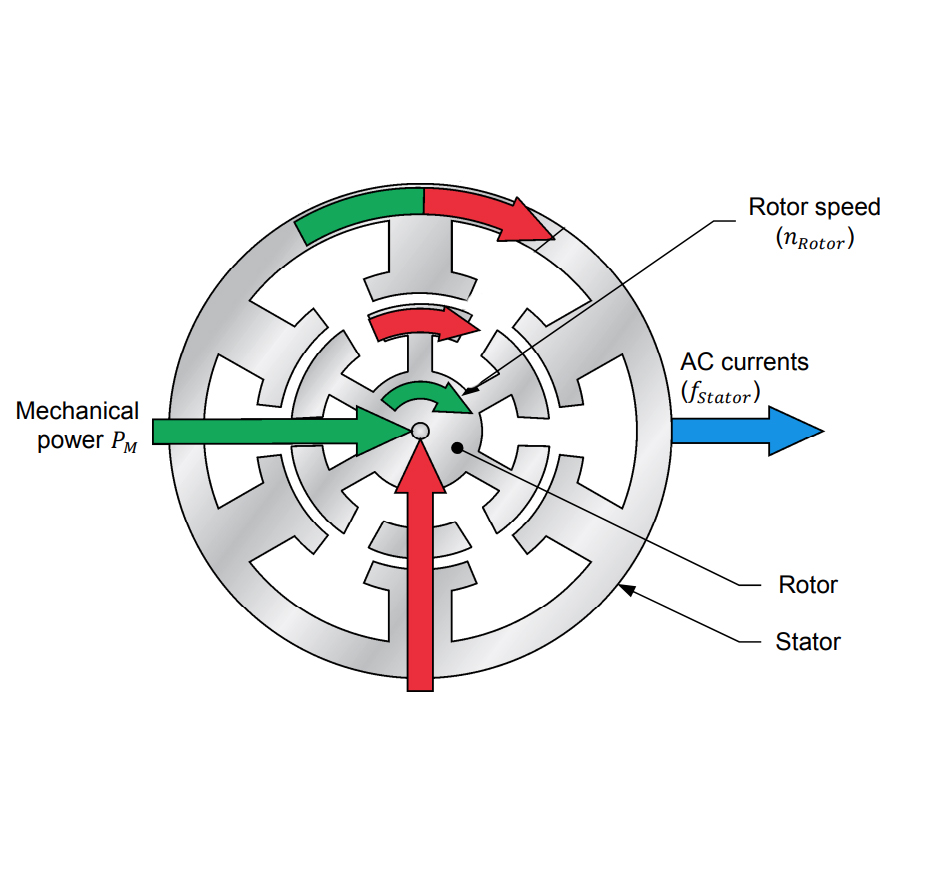
\includegraphics[width=2.85in]{imgs/dfigOP (2).jpg}
        \caption{Mechanical power imparted into rotor, which induces AC voltage with frequency $f_{stator}$}
    \end{figure}
\end{frame}

\begin{frame}{}
    \begin{figure}
        \centering
        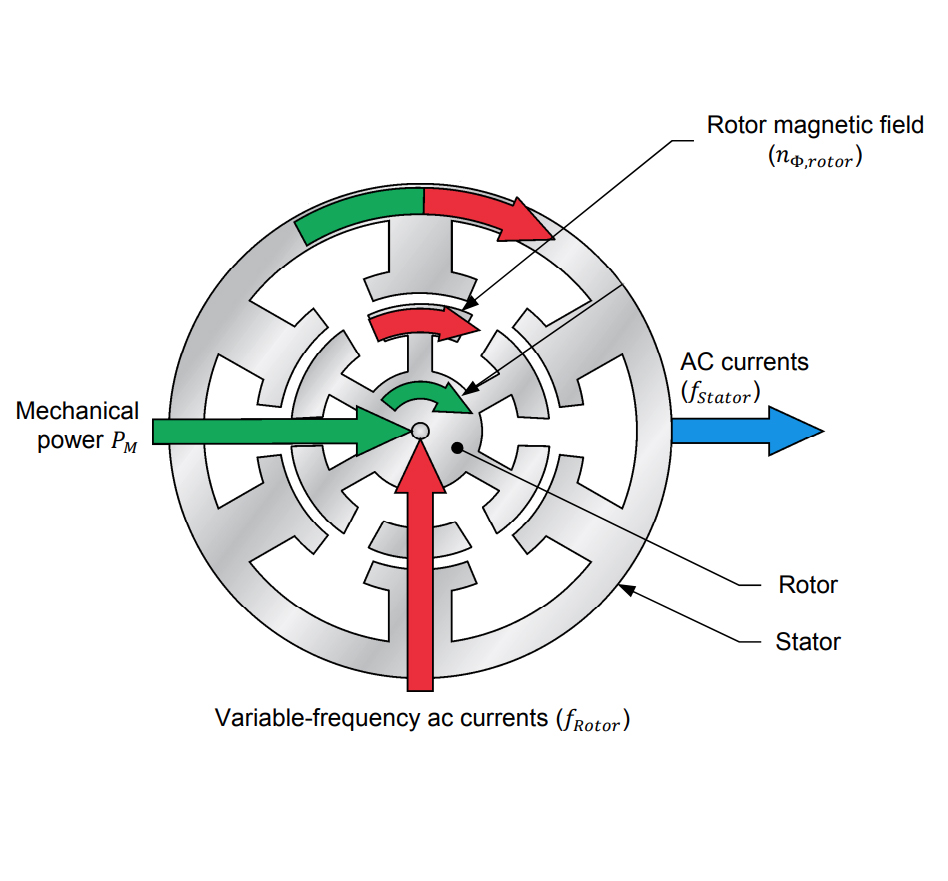
\includegraphics[width=2.85in]{imgs/dfigOP (3).jpg}
        \caption{Rotor's AC current frequency determines the speed of Rotor's magnetic field.}
    \end{figure}
\end{frame}



\begin{frame}{Animation time}
\begin{itemize}
    \item  \href{https://www.pengky.cn/zz-horizontal-axis-turbine/13-doubly-fed-wind-turbine-principle/rotor-magnetic-field.mp4}{DFIG principle with Magnetic field animation}
    

    \item \href{https://www.pengky.cn/zz-horizontal-axis-turbine/13-doubly-fed-wind-turbine-principle/doubly-fed-system.mp4}{DFIG Operation}


\vspace{0.5in}
\begin{quote}
\begin{center}
    
    \textcolor{mbrown}{``A picture is worth a thousand words, unless it’s an animation, then it’s priceless.'' \emoji{joy}}
    
\end{center}
\end{quote}

\end{itemize}
\end{frame}


\begin{frame}{}
    \begin{figure}
        \centering
        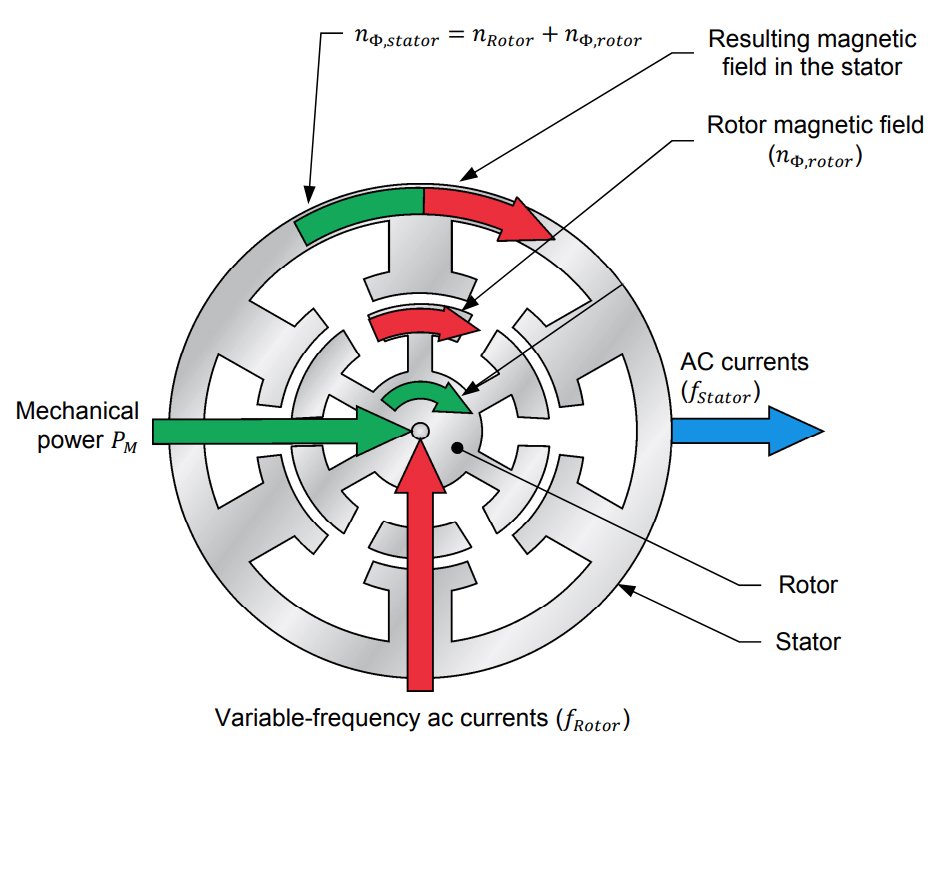
\includegraphics[width=2.85in]{imgs/dfigOP (4).jpg}
        \caption{Stator R.M.F. = Rotor's Mech. Speed + Rotor R.M.F. Speed}
    \end{figure}
\end{frame}

\begin{frame}{}
    \begin{figure}
        \centering
        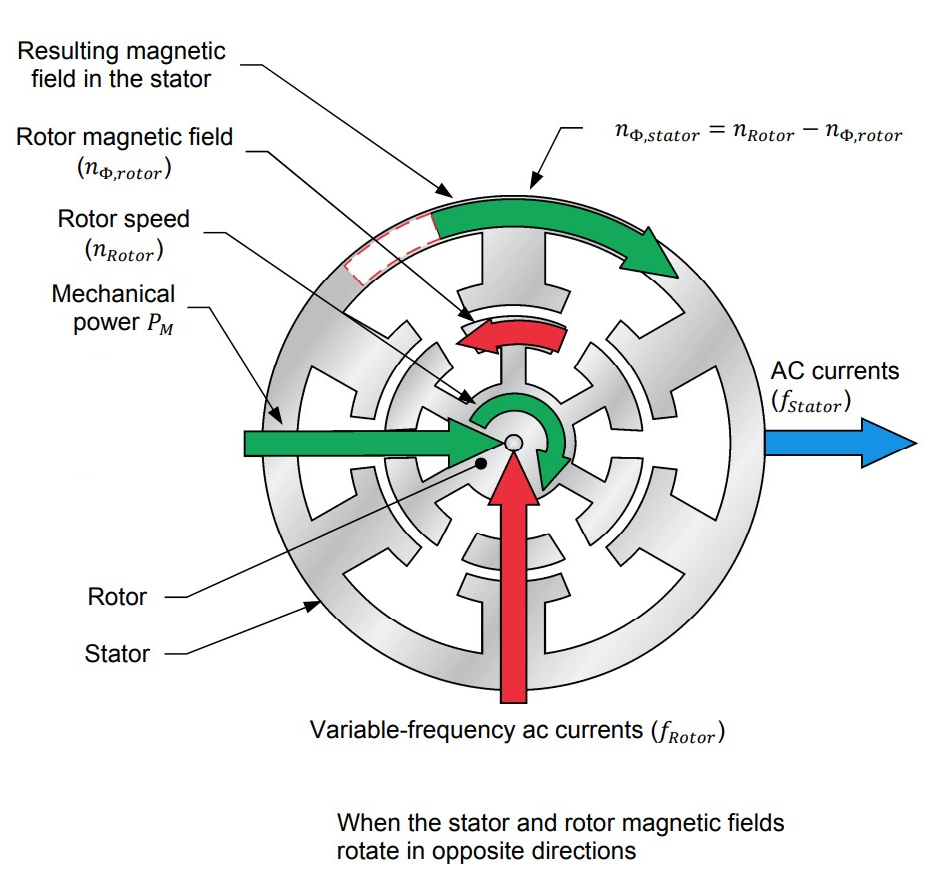
\includegraphics[width=2.85in]{imgs/dfigOP opposite.jpg}
        \caption{Stator R.M.F. = Rotor's Mech. Speed +  (- R.M.F. Speed)}
    \end{figure}
\end{frame}


\begin{frame}{Doubly-fed Induction Generator Empirical data}
    \begin{table}[h]
    \centering
    \rowcolors{2}{gray!25}{white} % Alternating row colors
    \resizebox{\textwidth}{!}{
    \begin{tabular}{|c|c|c|c|c|c|c|}
    \hline
    \rowcolor{gray!50} % Header row color
    \textbf{Speed (r/min)} & \textbf{Mechanical Power (W)} & \textbf{Stator Active Power (W)} & \textbf{Stator Reactive Power (var)} & \textbf{Rotor Frequency (Hz)} \\
    \hline
    1470 & 230.6 & 264.5 & 4.49 & 11 \\
    1500 & 235.4 & 267.0 & 4.55 & 10 \\
    1530 & 240.1 & 264.7 & -1.03 & 9 \\
    1559 & 244.5 & 264.7 & 5.53 & 8 \\
    1800 & 282.4 & 265.8 & 9.78 & 0 \\
    1919 & 300.8 & 264.4 & 2.25 & -4 \\
    1950 & 305.7 & 265.1 & -2.95 & -5 \\
    1980 & 310.5 & 265.5 & 0.57 & -6 \\
    2009 & 315.1 & 267.0 & 0.43 & -7 \\
    2040 & 319.9 & 267.0 & 0.91 & -8 \\
    2069 & 324.6 & 266.8 & -1.19 & -9 \\
    2099 & 328.7 & 267.3 & -3.22 & -10 \\
    \hline
    \end{tabular}
    }
    
    \caption{Table of Doubly-fed Induction Generator Results. from: Reference 1}
    
    \textbf{Machine data}:
    
    \begin{itemize}
        \item Poles $= 4$
        \item Grid frequency $= 60\, Hz$
        % \item Grid frequency $= 60\, Hz$
    \end{itemize}
    
    \end{table}
\end{frame}


\begin{frame}{Key Points}
\begin{itemize}
    
    \item A \textit{DFIG} functions as a \textit{variable-speed synchronous generator}, it can be adjusted by modifying the rotor frequency ($f_{\textit{rotor}}$).

    \item During periods of \textbf{low wind speeds}, the rotor frequency is increased, to match the synchronous grid frequency.

    \item Conversely, during \textbf{high wind speeds}, the rotor frequency is increased, but the direction of $Rotor_{R.M.F.}$ is reversed to counterbalance the high speed, matching the synchronous grid frequency. 

\end{itemize}
\end{frame}



\begin{frame}{Operational Range}
 \begin{columns}
\begin{column}{0.5\textwidth} 
    \begin{figure}
        \centering
        \fbox{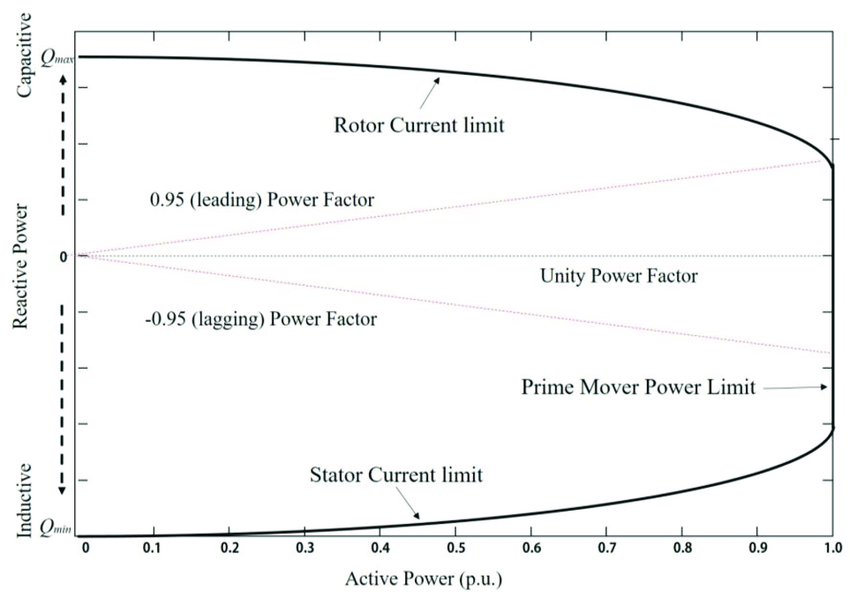
\includegraphics[width=2.2in]{imgs/capa.png}}
        \caption{Capability curve of DFIG}
    \end{figure}
    \end{column}
    
    \begin{column}{0.4\textwidth} % Adjust the width as needed
      \begin{itemize}
        \item It allows variation of $\pm \,30\%$ synchronous speed.

        \item Limits due to armature and field heating.
    
      \end{itemize}
    \end{column}
  \end{columns}
\end{frame}


\section{Control System}

\begin{frame}{Control principle}

\begin{itemize}
 \item  The control principle used is either the 

\begin{itemize}
    \item Two-axis current vector control 
    \item or Direct Torque Control D.T.C.
\end{itemize}

\item D.T.C. proved to be stable high reactive currents are required from generator.
\end{itemize}

\end{frame}



\begin{frame}{Vector control of DFIG}
    \begin{figure}
        \centering
        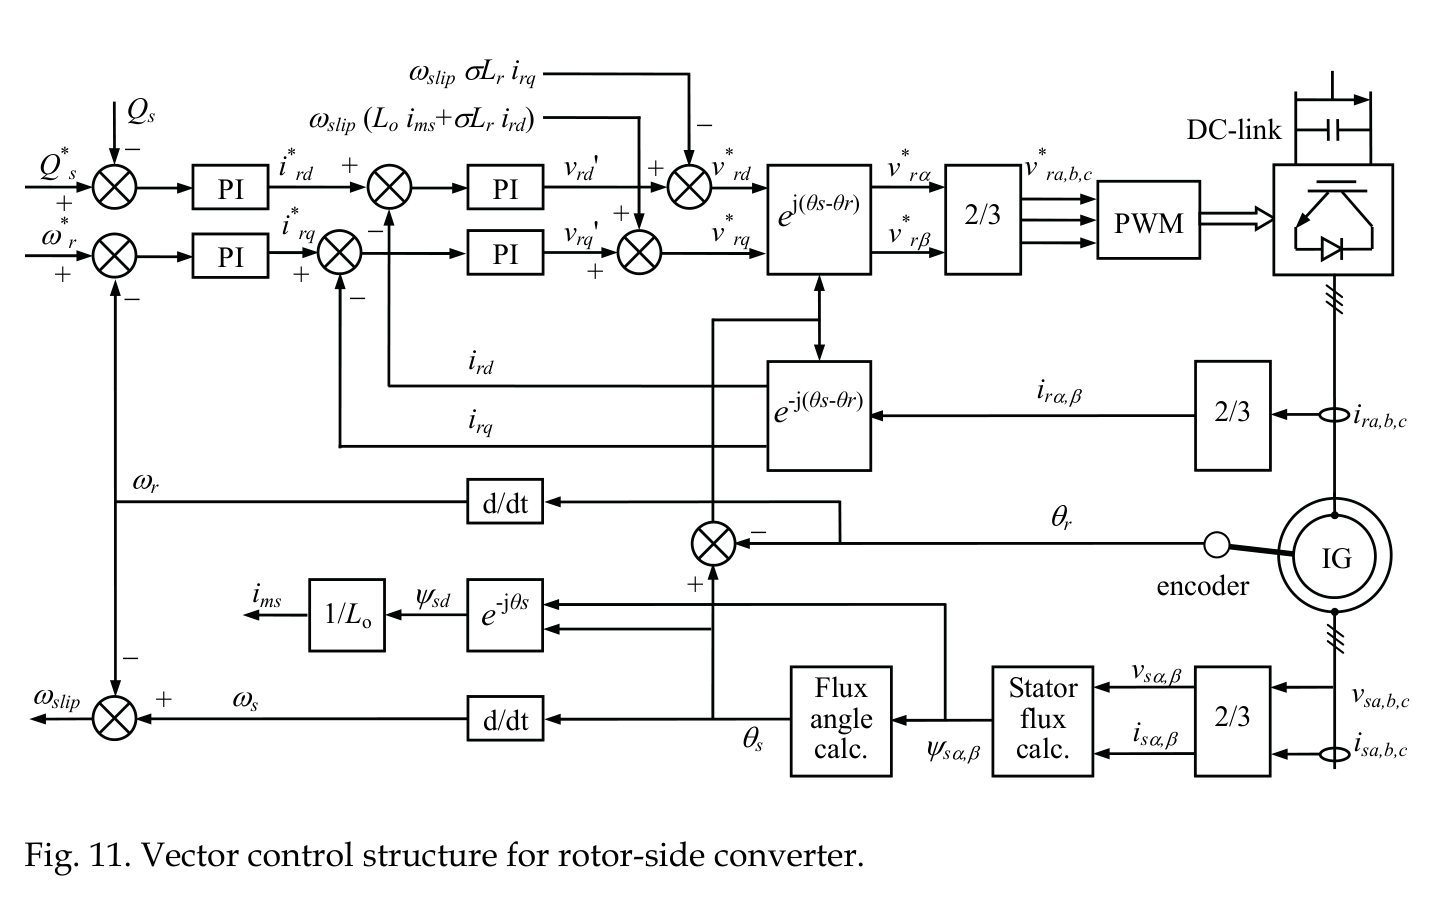
\includegraphics[width=4in]{imgs/rotorSideConv.png}
    \end{figure}    
\end{frame}



\begin{frame}{Direct torque control of DFIG}
    \begin{figure}
        \centering
        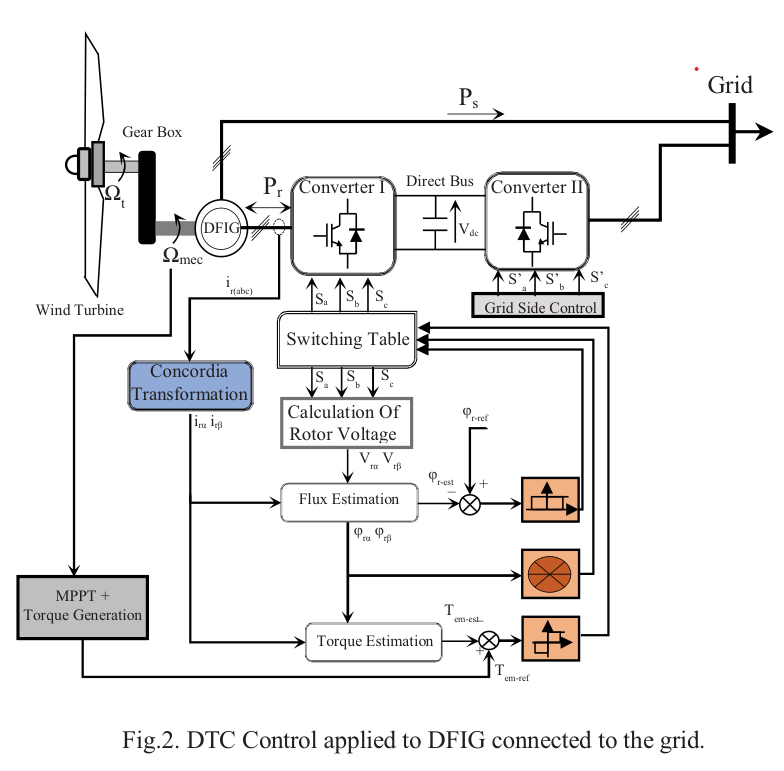
\includegraphics[width=3.2in]{imgs/DTCrotor.png}
    \end{figure}    
\end{frame}

\begin{frame}{Merits and Demerits of DFIGs}
  \begin{columns}[T]
    \column{0.5\textwidth}
    \begin{block}{Merits}
      \begin{itemize}
      \item Easy on the \textbf{gearbox}. (Reduced mechanical stress due to power system).
   
        \item Better fault ride-through capability. Whereas synchronous generator will \textbf{slip} when $V_{stator}$ falls below a threshold.
           \pause
        \item Smaller converter size (only about 30\% of the rated power).
        
        \item Ability to support grid voltage and frequency regulation.
      \end{itemize}
    \end{block}
    \column{0.5\textwidth}
    \begin{block}{Demerits}
      \begin{itemize}
        \item Complex power conversion circuitry.
        \item Slip ring and brush maintenance.
      \end{itemize}
    \end{block}
  \end{columns}
\end{frame}


\section{Acknowledgements}
\begin{frame}{References \emoji{book}}
    This presentation would not have been possible without the invaluable following:
    \vspace{0.1in}
    \begin{enumerate}
        \item \href{https://web.archive.org/web/20230526092355/https://labvolt.festo.com/downloads/86376_F0.pdf}{A \textbf{wonderful practical} introduction to DFIG from labvolt.festo.com}

        \item \href{https://www.pengky.cn/zz-horizontal-axis-turbine/13-doubly-fed-wind-turbine-principle/doubly-fed-wind-turbine-principle.html}{Peng DFIGs principle with \textbf{beautiful} animations}
      
        \item \href{https://www.wikiwand.com/en/Doubly_fed_electric_machine}{DFIG Wikipedia-Wikiwand}
        
        \item \href{https://new.abb.com/motors-generators/generators/generators-for-renewables/doubly-fed-generators}{ABB.com DFIGs}
        
        \item \href{https://www.youtube.com/watch?v=Fvc2I0L2vMU}{Evan Knapp video on DIFG}
        
        \item \href{https://explore.airgapflux.in}{My website - explore.airgapflux.in} (Additional resources on the subject)

    \end{enumerate}
\end{frame}



\begin{frame}{Tools used \emoji{wrench}}
    \begin{enumerate}
        \item Latex Beamer source code for this presentation can be found here: \href{https://github.com/200901002/DFIG-Seminar}{GitHub DFIG seminar Adhithya}.
        
        \item Adobe Photoshop was used to edit some of the images.

        \item \href{https://www.overleaf.com}{Overleaf.com}, which was used for preparing this presentation.
        
        \item Special thanks to LaTeX Beamer tools and the authors of the Singapore theme, whose contributions greatly improved the quality of this presentation.
    \end{enumerate}
    \vspace{0.2in}

    \begin{quote}
        \textcolor{mbrown}{``Education is the journey that transforms curiosity into knowledge and passion into expertise.''}
    \end{quote}

    \begin{center}
        {\Large{Thank you for your time \emoji{smile}}}
    \end{center}

    \begin{flushright}
        {\textbf{Adhithya}} \\
        Email \emoji{email}: \href{mailto:200901002@rajalakshmi.edu.in}{200901002@rajalakshmi.edu.in} \\
        LinkedIn \emoji{man}: \href{https://www.linkedin.com/in/adhithya-s-2a4338240/}{linkedin.com/in/adhithya-s-2a4338240}
    \end{flushright}
\end{frame}



\end{document}